\section{Medidas a 135ºC}
\label{sec:ResT135}

Considerando o problema com a variabilidade da temperatura ambiente também foram realizadas medidas na temperatura de 135°C, por ser a temperatura que a câmara térmica estabilizava. As medidas eram feitas pelo menos 30 minutos após a temperatura alvo ter sido atingida para se obter um valor mais consolidado.

As medidas nessa temperatura só começaram a ser feitas a partir de 14 horas de exposição, pelo fato de nos primeiros ciclos ter sido usado temperaturas mais baixas para verificar se haveriam danos críticos aos dispositivos, como descrito na Seção \ref{sec:MetEnsaios}.

A Figura \ref{fig:T135DE2} mostra as curvas das frequências normalizadas dos osciladores das placas  DE2 que foi estressada termicamente em relação ao tempo de exposição. Nela é visto que a degradação continuou, mesmo que pequena, até o fim dos ensaios, o que não podia ser observado na Figura \ref{fig:TAmbDE2} devido a variação da temperatura ambiente.

\begin{figure}[H]
    \centering
    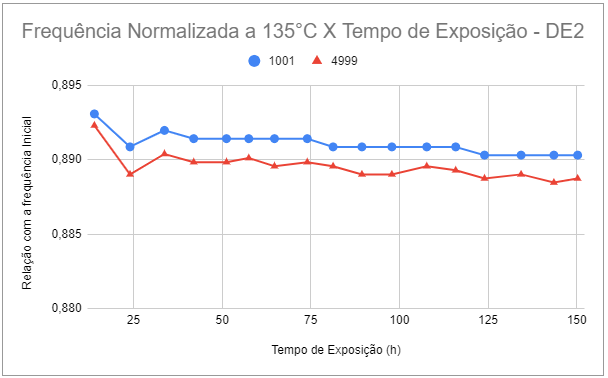
\includegraphics[scale=0.75]{figures/Resultados/T135DE2}
    \caption{Curva da DE2 a 135ºC. Fonte: O Autor}
    \label{fig:T135DE2}
\end{figure}

A Figura \ref{fig:T135ZedBoard} mostra as curvas para a ZedBoard, possuindo um comportamento semelhante ao discutido sobre a Figura \ref{fig:TAmbZedBoard}.

\begin{figure}[H]
    \centering
    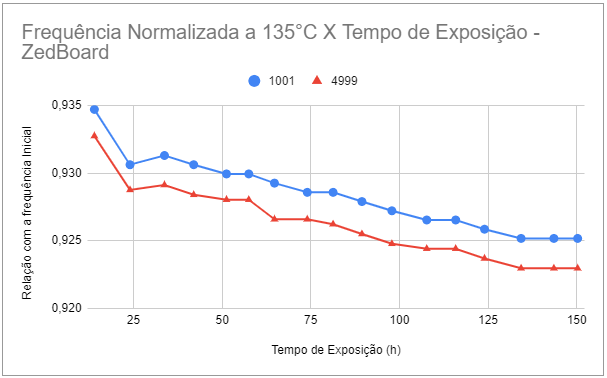
\includegraphics[scale=0.75]{figures/Resultados/T135ZedBoard}
    \caption{Curva da ZedBoard a 135ºC. Fonte: O Autor}
    \label{fig:T135ZedBoard}
\end{figure}

A Figura \ref{fig:T135Ambas} mostras as duas as curvas das Figura \ref{fig:T135DE2} e \ref{fig:T135ZedBoard} juntas no mesmo gráfico.

\begin{figure}[H]
    \centering
    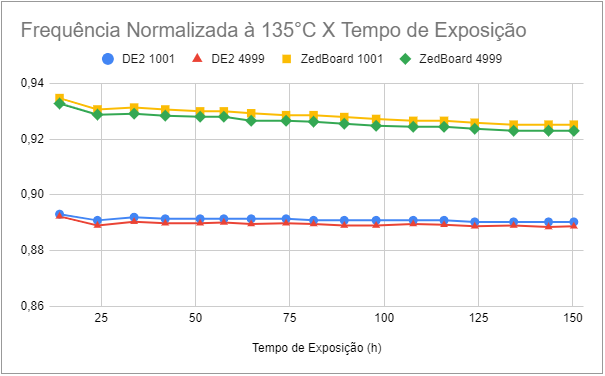
\includegraphics[scale=0.75]{figures/Resultados/T135Ambas}
    \caption{Comparação das duas placas a 135ºC. Fonte: O Autor}
    \label{fig:T135Ambas}
\end{figure}

A Tabela \ref{tab:FreqT135} mostra as frequências iniciais e finais dos osciladores das duas placas que foram estressadas.

\begin{table}[H]
\centering
\caption{Frequências iniciais e finais dos osciladores a 135°C.}
\begin{tabular}{l|cccc|}
\cline{2-5}
 & \multicolumn{4}{c|}{\textbf{Frequência (kHz)}} \\ \cline{2-5} 
 & \multicolumn{2}{c|}{\textbf{Altera DE2}} & \multicolumn{2}{c|}{\textbf{ZedBoard}} \\ \cline{2-5} 
 & \multicolumn{1}{c|}{\textbf{1001}} & \multicolumn{1}{c|}{\textbf{4999}} & \multicolumn{1}{c|}{\textbf{1001}} & \textbf{4999} \\ \hline
\multicolumn{1}{|c|}{\textbf{Inicial}} & \multicolumn{1}{c|}{1612} & \multicolumn{1}{c|}{325,6} & \multicolumn{1}{c|}{1374} & 257,9 \\ \hline
\multicolumn{1}{|c|}{\textbf{Final}} & \multicolumn{1}{c|}{1607} & \multicolumn{1}{c|}{324,3} & \multicolumn{1}{c|}{1360} & 255,2 \\ \hline
\end{tabular}
\label{tab:FreqT135}
\end{table}

As curvas das Figuras \ref{fig:T135DE2} e \ref{fig:T135ZedBoard} apresentam um comportamento semelhante às curvas da Seção \ref{sec:ResTAmb}, mostrando que a tendência do FPGA da ZedBoard degradar mais que o da DE2 continua independente da temperatura. Porém, essas medidas não podem ser comparadas de nenhuma forma com as medidas das placas de controle, já que elas sempre operaram na temperatura ambiente.
